\section{Pressure}
\label{sec:dsmc_pressure}
Pressure skits a blingin role up in tha field of fluid flow fo' realz. An applied heat difference (which gives a net force) is probably what tha fuck induces tha flow, up in addizzle ta bein a blingin property of tha fluid. Y'all KNOW dat shit, muthafucka! Da rap bout heat gotz nuff both how tha fuck we \textit{define} tha pressure, n' we \textit{measure} it up in a DSMC simulation. I aint talkin' bout chicken n' gravy biatch fo' realz. And of course how tha fuck we induce flow up in tha simulation. I aint talkin' bout chicken n' gravy biatch. Well shiiiit, it turns up dat DSMC satisfies tha ideal gas equation of state, so given constant temperature, tha local heat is proportionizzle ta tha local densitizzle fo' realz. A heat difference, or heat gradient, would then require a similar gradient up in tha density. This is hard as fuck ta obtain up in a system wit periodic boundary conditions cuz $\rho(x=0) = \rho(x=L)$ fo' a system of length $L$. Instead we will derive a relation between tha heat gradient n' a cold-ass lil correspondin constant force which we will use ta induce flow up in tha simulations. 
\subsection{Equation of state}
\label{sec:dsmc_eos}
Da free \textit{modules} up in a DSMC program is tha collision operator $\mathcal C$ n' tha move operator $\mathcal M$ which straight-up (stochastically) determine tha time evolution of tha system. For systems wit pairwise interactions (like fuckin hard spheres or tha Lennard-Jones potential which we hook up in section \ref{sec:md_model}), tha heat may be defined as (see appendix \ref{sec:pressure_derivation} fo' a thugged-out derivation)
\begin{align}
	P = \rho_nk_BT + \frac{1}{3V}\bigg\langle \sum_{i<j} \vec F(\vec r_{ij})\cdot \vec r_{ij}\bigg\rangle,
\end{align}
where tha straight-up original gangsta term is tha ideal gas heat whereas tha second term is called tha virial of tha heat yo. Here $\vec F(\vec r_{ij})$ is tha force between particle $i$ n' $j$, n' $\vec r_{ij}$ is they relatizzle distance. In DSMC our phat asses aint gots tha details bout tha forces yo, but we can formulate a similar expression rockin dat tha force is tha chizzle up in momentum per time
\begin{align}
	P = \rho_nk_BT + \frac{1}{3Vt}\sum_\text{all collisions} m\Delta \vec v_{ij}\cdot \vec r_{ij},
\end{align}
where $\Delta \vec v_{ij}$ is tha chizzle of velocitizzle of one of tha particlez durin a cold-ass lil collision\cite{garcia1997direct}. In tha collision model our crazy asses have used, there be no correlation between tha chizzle up in velocitizzle $\Delta \vec v_{ij}$ n' tha displacement vector $\vec r_{ij}$ between tha particles
\begin{align}
	\left\langle \Delta \vec v_{ij}\cdot \vec r_{ij}\right\rangle = 0,
\end{align}
so tha expression fo' tha heat is reduced ta dat of a ideal gas
\begin{align}
	P = \rho_n k_BT.
\end{align}
Since tha main focuz of dis thesis is ta study dilute gases where tha ideal gas be a phat approximation, dis collision model is sufficient. For dense gases, or liquids, it is possible ta apply collision models dat yieldz other equationz of state \cite{garcia1997direct}.
\subsection{Measurin pressure}
Since tha gas satisfies tha ideal gas equation of state, dis iz of course how tha fuck we measure tha pressure
\begin{align}
	P = \rho_n k_BT,
\end{align}
since we already know how tha fuck ta calculate tha densitizzle n' tha temperature. Da local heat iz of course found by rockin tha local jointz of tha densitizzle n' temperature.
\subsection{Applyin a heat gradient}
\label{sec:dsmc_applying_pressured_grad}
In order ta induce flow up in a system, it is common ta apply a heat gradient fo' realz. A heat gradient means dat there acts a nonzero net force on any volume element $\dm V$ up in tha system. In continuum models like tha NSE (see section \ref{sec:theory_of_fluids_euler_navier}), tha heat (and hence tha heat gradients) is incorporated as boundary conditions where heat is specified at given points fo' realz. A typical boundary condizzle is $P(x=0) = P_0$ n' $P(x=L) = P_L$ yo, but as we already mentioned, periodic boundary conditions be a problem since tha points is tha straight-up same point. Instead we will use scams from continuum mechanics ta relate a given heat gradient ta a cold-ass lil constant force which we will apply on all particlez up in tha system. In tha literature, dis is often called gravitizzle driven flow.

We peep a volume element of size $\Delta V = \Delta x\Delta y\Delta z$ up in a cold-ass lil channel wit a cold-ass lil continuous fluid n' a heat gradient up in tha $x$-direction, peep figure \ref{fig:pressure_gravity_equivalent}. 
\begin{figure}[h]
\begin{center}
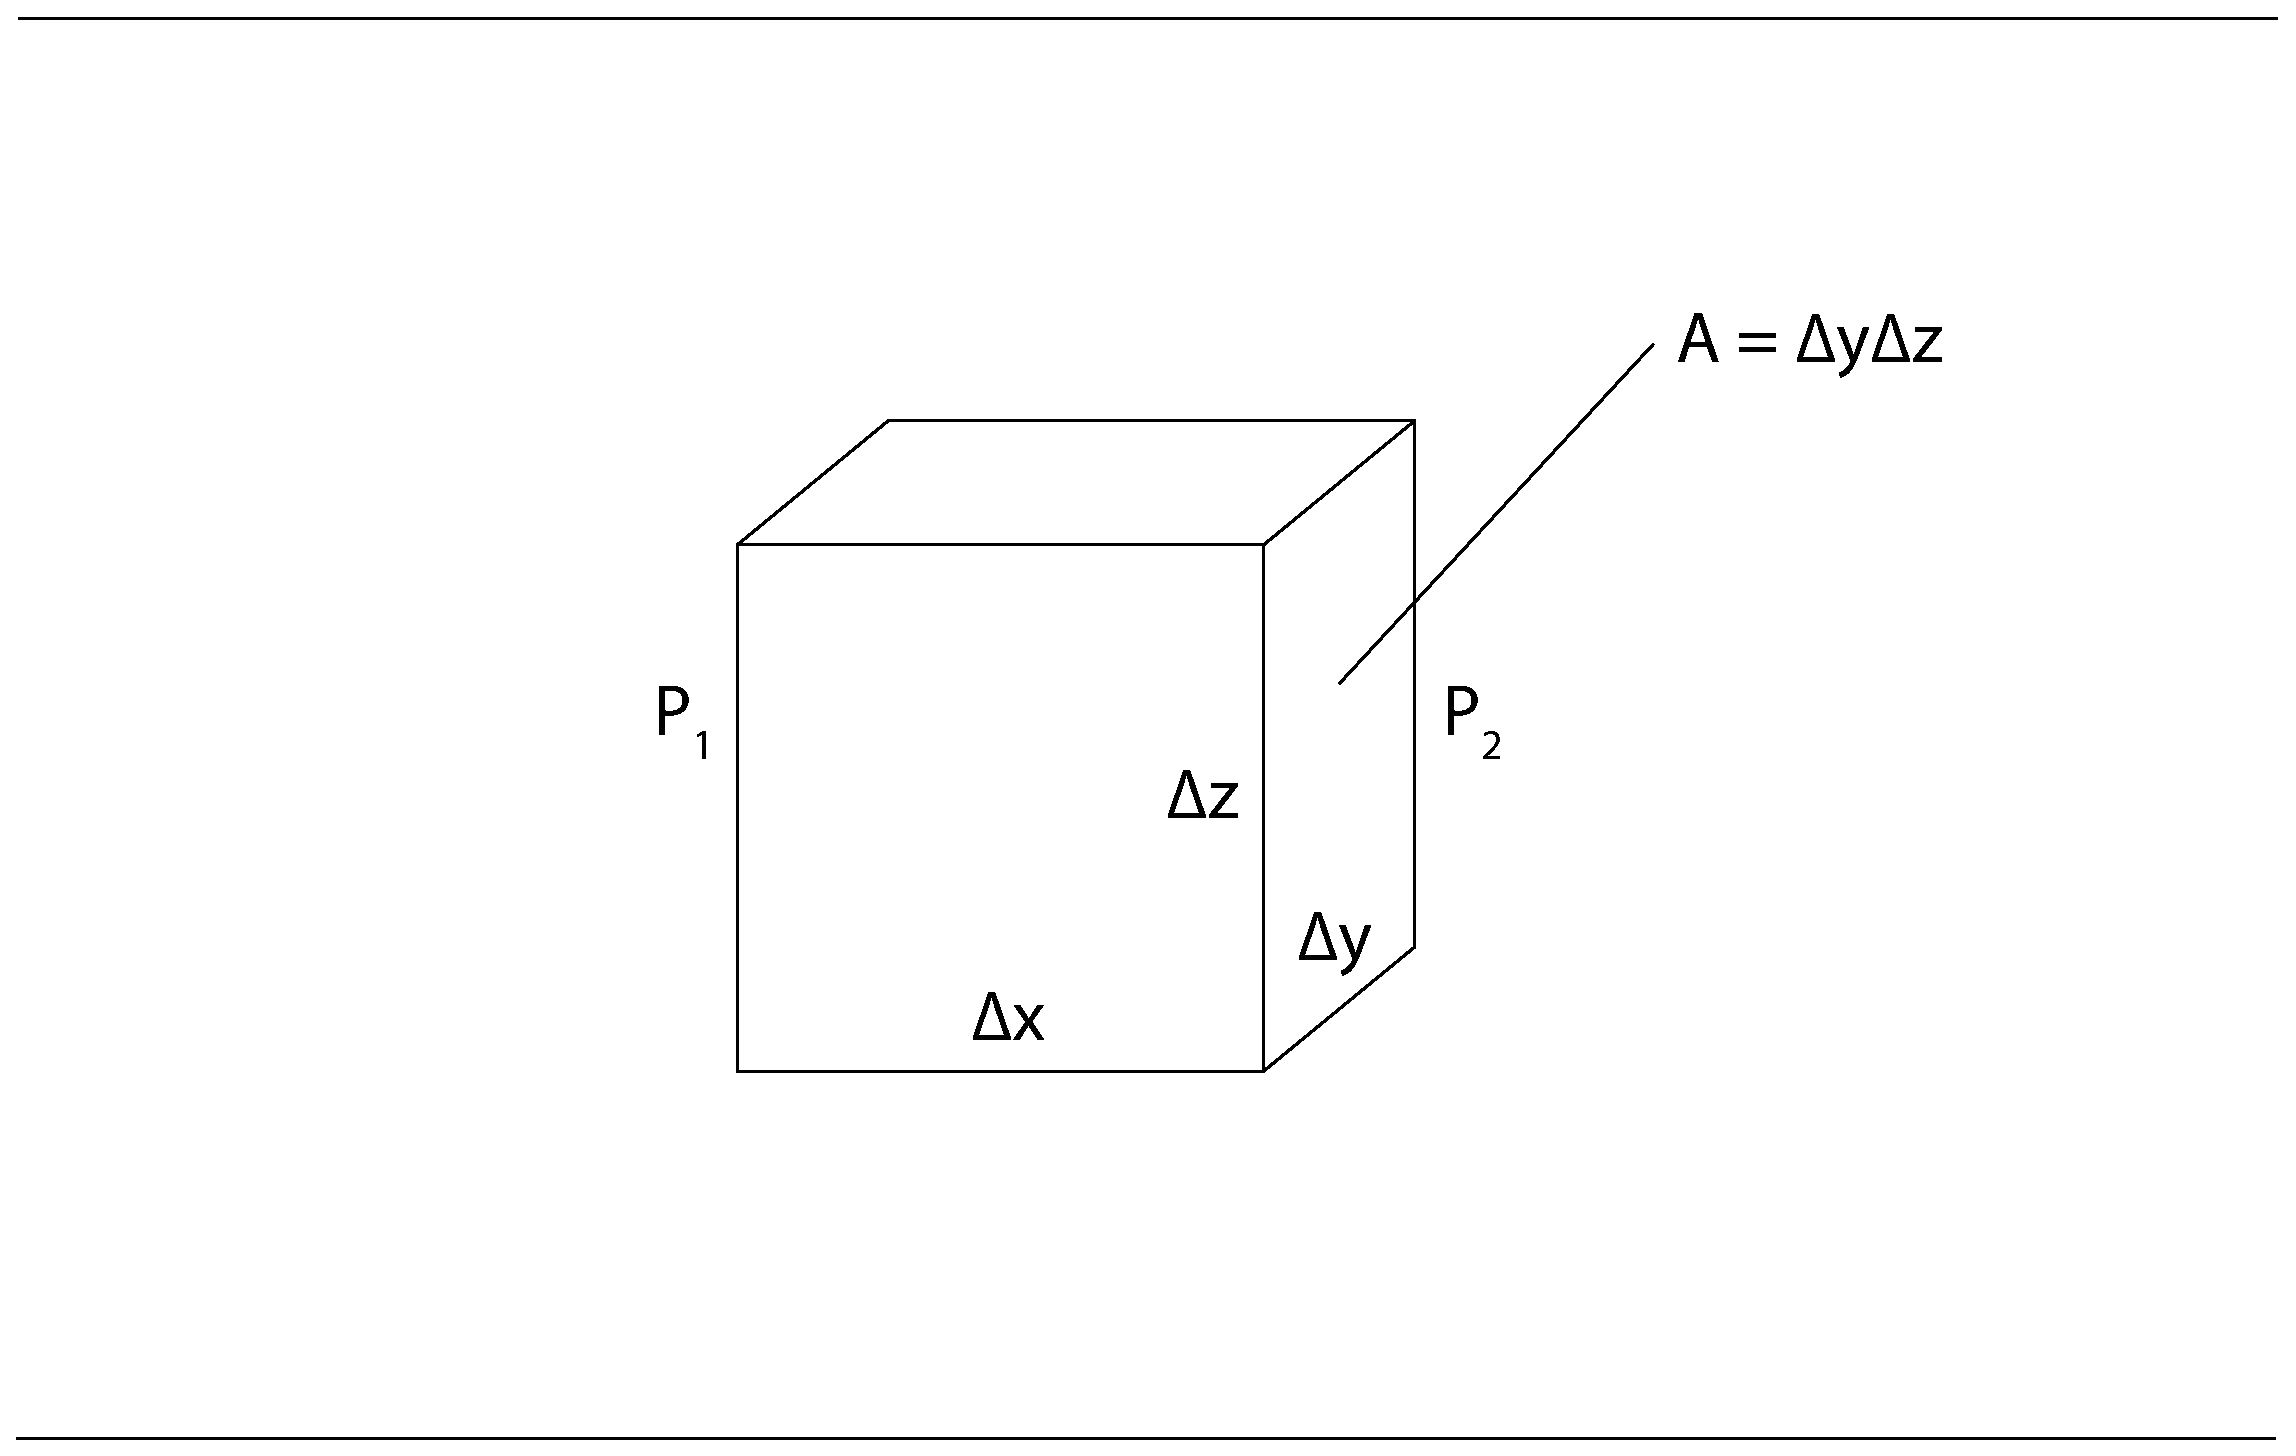
\includegraphics[width=\textwidth, trim=0cm 0cm 0cm 0cm, clip]{DSMC/figures/pressure_to_gravity.eps}
\end{center}
\caption{Da net force actin on tha volume element $\Delta V = \Delta x\Delta y\Delta z$ up in tha $x-$direction is given by tha heat difference times area $A(P_2 - P_1) = \Delta y\Delta z\Delta P$.}
\label{fig:pressure_gravity_equivalent}
\end{figure}
Da net force actin on tha volume element up in tha $x-$direction is
\begin{align}
	F = P_2\Delta y\Delta z - P_1\Delta y\Delta z = \Delta y\Delta z\Delta P,
\end{align}
where $\Delta P = P_2 - P_1$. We aim ta find a cold-ass lil constant force $F=mg$ bein equivalent ta dat of tha heat difference. Given a acceleration $g$, tha force is then
\begin{align}
	F = mg = \rho_m \Delta V g.
\end{align}
We aim ta find a gangbangin' force equal ta tha one from tha heat difference
\begin{align}
	F = \Delta y\Delta z\Delta P = \Delta V \frac{\Delta P}{\Delta x},	
\end{align}
which gives tha relation
\begin{align}
	\label{eq:acceleration_to_pressure_difference}
	g = \frac{\Delta P}{\rho_m\Delta x}.
\end{align}
In simple geometries like a tube, tha behavior of tha flow fo' both heat models should be similar. Shiiit, dis aint no joke. But fuck dat shiznit yo, tha word on tha street is dat fo' disordered systems wit regions dat can \textit{trap} particles, we can expect some effects dat will affect tha fluid flow up in a non-physical way fo' realz. An example is shown up in figure \ref{fig:gravity_problem} where a gas driven by a cold-ass lil constant acceleration up in tha x-direction is ghon be slowed down up in tha area marked gray. In a gas driven by a real heat difference, we expect a net force along tha channel up in all regions.
\begin{figure}[h]
\begin{center}
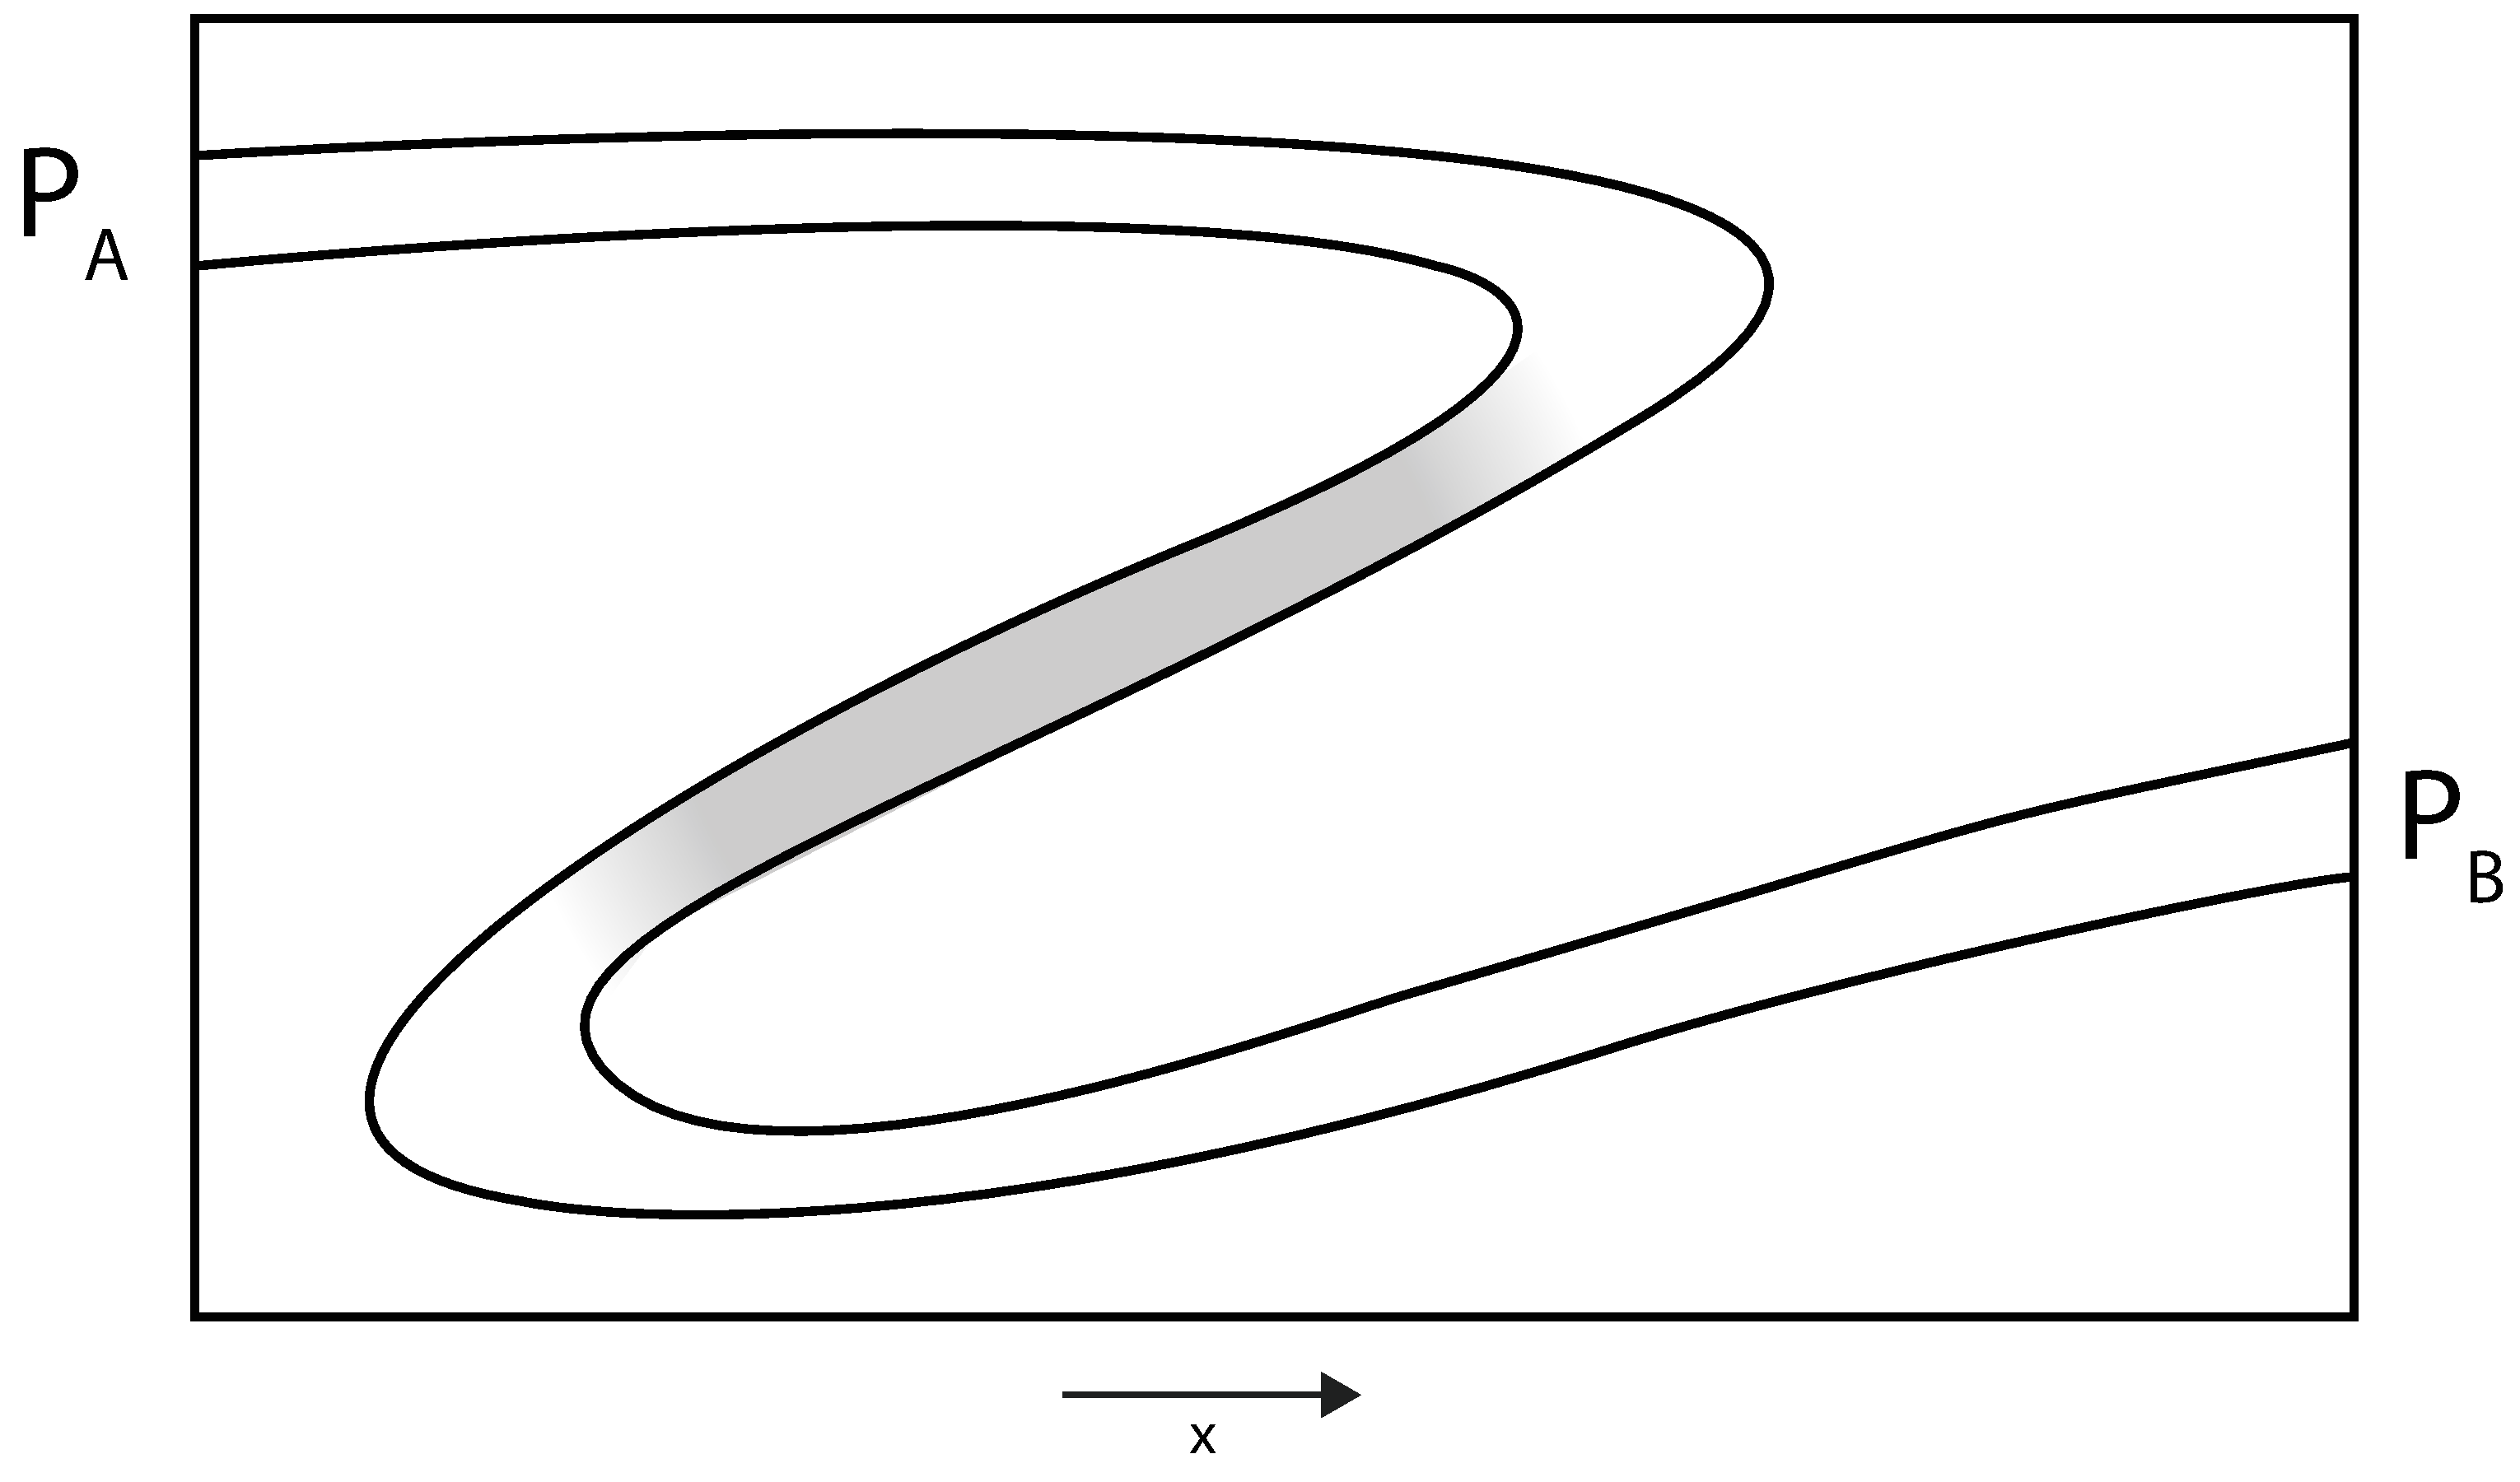
\includegraphics[width=0.7\textwidth, trim=0cm 0cm 0cm 0cm, clip]{DSMC/figures/gravity_problem.eps}
\end{center}
\caption{Flow induced by a cold-ass lil constant acceleration aint gonna reproduce erect flow behavior when tha gas up in a larger part (marked gray) of tha channel flows up in tha opposite direction of tha force. In a \textit{real} pressure-driven flow, tha net force on tha gas will point along tha expected flow direction, also up in tha gray marked area, whereas tha acceleration-driven flow is ghon be slowed down.}
\label{fig:gravity_problem}
\end{figure}
We can now obtain a thugged-out desired heat difference all up in equation \eqref{eq:acceleration_to_pressure_difference} n' apply dat acceleration ta all particlez each timestep.